\documentclass{report}

\usepackage[utf8]{inputenc}
\usepackage{natbib} % to use bibliography
\usepackage{graphicx} % to include graphics
\usepackage{subcaption} % to include sub graphics
\usepackage{amsmath} % to include extended mathematics
\usepackage[breaklinks]{hyperref} % to include links
\usepackage[acronym, toc]{glossaries} % to include a glossary
\usepackage{fancyhdr} % to style header and footer
\usepackage[nottoc]{tocbibind} % adds bibliography to ToC
\usepackage{listings} % to include code snippets
\usepackage{xcolor} % to colorize source code
\usepackage{array} % to define custom column types

% define column types with a fixed length
\newcolumntype{L}[1]{>{\raggedright\let\newline\\\arraybackslash\hspace{0pt}}m{#1}}
\newcolumntype{C}[1]{>{\centering\let\newline\\\arraybackslash\hspace{0pt}}m{#1}}

% set resources path
\graphicspath{ {./resources/} }

% create hyperlinks for ToC
\hypersetup{
    linktoc=all,
}

% define colors for code
\definecolor{commentsColor}{rgb}{0.497495, 0.497587, 0.497464}
\definecolor{keywordsColor}{rgb}{0.000000, 0.000000, 0.635294}
\definecolor{stringColor}{rgb}{0.558215, 0.000000, 0.135316}

\lstset{ %
  backgroundcolor=\color{white},   % choose the background color
  basicstyle=\ttfamily\footnotesize,        % the size of the fonts that are used for the code
  breakatwhitespace=false,         % sets if automatic breaks should only happen at whitespace
  breaklines=true,                 % sets automatic line breaking
  captionpos=b,                    % sets the caption-position to bottom
  commentstyle=\color{commentsColor}\textit,    % comment style
  deletekeywords={...},            % if you want to delete keywords from the given language
  escapeinside={\%*}{*)},          % if you want to add LaTeX within your code
  extendedchars=true,              % lets you use non-ASCII characters; for 8-bits encodings only, does not work with UTF-8
  frame=tb,	                   	   % adds a frame around the code
  keepspaces=true,                 % keeps spaces in text, useful for keeping indentation of code (possibly needs columns=flexible)
  keywordstyle=\color{keywordsColor}\bfseries,       % keyword style
  language=Python,                 % the language of the code (can be overrided per snippet)
  otherkeywords={*,...},           % if you want to add more keywords to the set
  numbers=left,                    % where to put the line-numbers; possible values are (none, left, right)
  numbersep=5pt,                   % how far the line-numbers are from the code
  numberstyle=\tiny\color{commentsColor}, % the style that is used for the line-numbers
  rulecolor=\color{black},         % if not set, the frame-color may be changed on line-breaks within not-black text (e.g. comments (green here))
  showspaces=false,                % show spaces everywhere adding particular underscores; it overrides 'showstringspaces'
  showstringspaces=false,          % underline spaces within strings only
  showtabs=false,                  % show tabs within strings adding particular underscores
  stepnumber=1,                    % the step between two line-numbers. If it's 1, each line will be numbered
  stringstyle=\color{stringColor}, % string literal style
  tabsize=2,	                   % sets default tabsize to 2 spaces
  title=\lstname,                  % show the filename of files included with \lstinputlisting; also try caption instead of title
  literate={\ \ }{{\ }}1,
  columns=fixed                    % Using fixed column width (for e.g. nice alignment)
}

% rename bibliography to references
\renewcommand{\bibname}{References}

% define header and footer
\pagestyle{fancy}
\fancyhf{} % clear all
\renewcommand{\chaptermark}[1]{\markboth{#1}{}}
\renewcommand{\sectionmark}[1]{\markright{#1}}
\lhead{\rightmark}
\rhead{\textbf{\leftmark}}
\cfoot{\thepage}

\title{\textbf{Nero} - A named-entity recognition model for insurances}
\author{Yves Beutler}
\date{January 2020}

% initialize glossary
\makeglossaries
\newglossaryentry{mobi24}
{
    name=mobi24,
    description={the 24h assistance and emergency call center of Swiss Mobiliar}
}

\newglossaryentry{infomobi}
{
    name=infomobi,
    description={mailbox from info@mobiliar.ch used as data source}
}

\newglossaryentry{meinemobi}
{
    name=meinemobi,
    description={mailbox from meinemobiliar@mobiliar.ch used as data source}
}

\newglossaryentry{Duden}
{
    name=Duden,
    description={a spelling dictionary of the German language}
}

\newglossaryentry{diacritic}{
    name=diacritic,
    description={a sign added to a letter to indicate a different pronunciation}
}

\newglossaryentry{Protekta}
{
    name=Protekta,
    description={the legal protection insurance which is part of Swiss Mobiliar}
}

\newacronym{ner}{NER}{named-entity recognition}

\newacronym{nlp}{NLP}{natural language processing}

\newacronym{ml}{ML}{machine learning}

\newacronym{iob}{IOB}{Inside-outside-beginning}

\newacronym{pst}{PST}{Personal Storage Table}

\newacronym{kpi}{KPI}{key performance indicator}

\newacronym{ne}{NE}{named entity}

\newacronym{rnn}{RNN}{recurrent neural network}

\newacronym{dnn}{DNN}{deep neural network}

\newacronym{bfh}{BFH}{Bern University of Applied Sciences}

\newacronym{mlp}{MLP}{multilayer perceptron}

\begin{document}

\maketitle

\tableofcontents
\listoffigures
\listoftables
\lstlistoflistings

% insert chapters here
\chapter{Introduction}

Everyday, humans generate a huge set of information while interacting with the internet, especially since the era of the
Internet of Things (IoT). This data is often discarded, sometimes be logged, but even then in most
cases there is no further usage. Tasks like storing data and logging are considered tedious and receive little attention
apart from the initial programming work.

However, this is precisely the kind of data which is relevant for data science like the optimisation of an existing
business process with a cognitive model or the exploration of lucrative new business fields to invest in.

\section{Project Overview}

Mobi24 is an assistance and emergency call centre founded by the Swiss Mobiliar in 1997. It's the initial contact point for
clients and potential future clients. Most of the in-going requests are insurance related subjects. The purpose of
this bachelor thesis is the creation of a natural language model for named-entity recognition in the insurance context
based on client data from Mobi24. There already exist several pretrained models which are free to use, but just a few of them are
capable of dealing with the German language and none of them are trained with insurance data. In the future, the model from this thesis
should help the data scientists at Swiss Mobiliar for their own specific \acrshort{nlp}\footnote{Natural Language Processing deals
with the understanding of human languages} tasks. Currently the most interesting named entities for Swiss Mobiliar are the
people's names and their addresses.

\subsection{Benefits}

A reasonable \acrshort{ner} model will give the Swiss Mobiliar several benefits in understanding natural language and thereby
offering an even better service to its customers. The model will be available as a python library in the Swiss Mobiliar
repository so that Data Scientists can use it in their own projects.

Due to limited time resources the final model will only recognise names and addresses. However, it's possible to extend the list
of named entities with new values like phone numbers or insurance polices.

\subsubsection{Parameter Space and Complexity}

The main advantage of such a model is to create suitable data to reduce the parameter space of any other language model. The
size of the parameter space is defined by the used vocabulary. A varied vocabulary needs a much larger parameter space than
a smaller one to make plausible predictions. The number of layers, each layer's size and type are important indices to the
resulting size of the parameter space. There are more connections in a \acrshort{rnn} than in a \acrshort{dnn}, therefore
there are much more parameters in the \acrlong{rnn} if both networks are the exact same size.

With the reduced parameter space, the size of the model itself and it's training duration gets minimised. Especially if you want
to develop micro services, a lightweight and therefore fast model is required to satisfy customers needs.

Table \ref{tbl:param-space} shows, that the reduced vocabulary consists of much less tokens than the original one. In this
case it uses only $\frac{4}{7}$ of the tokens to express nearly the same amount of information. For a model, which wants to learn
user's intents and doesn't need the plain facts, this would be a real advantage. Of course there are plenty of other examples.

\begin{table}[h!]
    \centering
    \begin{tabular}{|l|c|c|c|c|c|c|c|}
        \hline
        \textbf{Default} & Sherlock & Holmes & lives & at & 221b & Baker & Street. \\
        \hline
        \textbf{Reduced} & PER & lives & at & LOC & & & \\
        \hline
    \end{tabular}
    \caption{Comparison of two sentences}
    \label{tbl:param-space}
\end{table}

\subsubsection{Anonymisation}

It's important to keep in mind that real anonymisation isn't possible. After data is being de-identified\footnote{The process
of anonymising personal data} it can be used and shared without the restrictions of data protection laws. Sharing research data
across institutions boosts the development of scientific inventions. The problem is that the data only seems to be anonymised. In
fact, there is a high chance to recognise individuals if the data is being populated with additional data sources \cite{rocher19}.
Imagine a de-identified insurance case about a car accident. There's the possibility to simply search news sites for car accidents at the concrete date to get personal information about the vehicle type or even the owner.

Nevertheless, the \acrshort{ner} model will be used to create anonymised data. The anonymised data could be used for demonstration
purposes. Even training in a cloud-based infrastructure would be significantly easier because of less restrictions from data policies. All data processed by the \acrshort{ner} model can be freely distributed across Swiss Mobiliar.

Instead of removing personal information there is also the opportunity to replace named entities with fictional values. The data
would look correct but isn't mirroring the reality and thus can be shared again. Although this approach may confuse users which
aren't aware of the fact that the entities are fictional it's worth mentioning. An advantage is that if a \acrshort{ne} was not
recognised and anonymised, the user would not know.

\subsubsection{Form Completion}

In information extraction, such a model can be useful to localise user data and complete a form with the extracted parts. If
you combine the model with an intent classifier\footnote{A model to predict user intents, widely used in smart assistants},
a very powerful combination arises \cite{jain18}. You could create pre-filled insurance offers from client requests. This would
speed up the process and may result in more sales. Swiss Mobiliar is currently doing research on chat bot for assisted claims
management, including damage classifier and automated suggestions.

\subsection{Objectives}

For a successful completion of the bachelor thesis several deliverables need to be offered to the stakeholders. Additionally
to this document there should exist a functioning language model with an anonymized training data set. This training set
should have an appropriate size for training the model and comparing the different outcomes. The source code should be
written under consideration of the commonly known software engineering and design patterns. The model is developed
iteratively with one or more baseline models at beginning. The goal is to optimise the model with every new approach to
get the highest possible recognition rate.

From an administrative point of view there needs to be a presentation in the middle of January. Furthermore an abstract, used
for the \acrshort{bfh} publication of all bachelor theses, a poster of size A3, and a short movie clip are expected.

\subsection{Stakeholders}

There are several stakeholders interested in the outcome of this project. There is the Swiss Mobiliar and especially its data
scientists, who want to reuse the trained NLP model for their own projects. On the other hand, there is the \acrlong{bfh} which
is demanding a satisfactory thesis for awarding me with the bachelor's degree in computer science. Last but not least, I act as
a stakeholder as well and I want to dig deeper in the field of data science and learn as much as possible.

It will be challenging to satisfy all these different stakeholders to an adequate level. Swiss Mobiliar is very focused on the
resulting model whereas the \acrshort{bfh} is more interested in the overall project, including time and project management.

\subsection{Submission Deadlines}

This bachelor thesis is carried out in compliance with various deadlines. Table \ref{tbl:deadlines} gives an insight about the most
relevant milestones and when they should be delivered to the stakeholders.

\begin{table}[ht!]
    \centering
    \begin{tabular}{|l|l|}
        \hline
        \textbf{Date} & \textbf{Submissions and Milestones} \\ [0.5ex]
        \hline
        16.09.2019 & Begin of semester, project kick off \\
        03.01.2020 & Submission of poster (A3) \\
        16.01.2020 & Submission of report, movie clip \\
        17.01.2020 & Presentation at BFH Techday \\
        17.01.2020 & Poster exhibition \\
        07.02.2020 & Grading conference \\
        06.03.2020 & Graduation party \\ [1ex]
        \hline
    \end{tabular}
    \caption{Most important (submission) dates}
    \label{tbl:deadlines}
\end{table}

\subsection{Data Privacy Protection}

All used examples and data snippets in this document are anonymised to protect the privacy of Swiss Mobiliar's clients. All names
and addresses are either cropped out of the original text or purely fictional.

\section{Data Sources}
\label{chap:data-source}
The future NLP model relies on two distinctive data sources. In detail, there is a single \emph{Personal Storage Table (.pst)
\footnote{An open proprietary file format by Microsoft used to store copies of messages}} for the email mailboxes
\emph{info@mobiliar.ch} and \emph{meinemobiliar@mobiliar.ch}. For a better understanding, the two data sources are called
\emph{\gls{infomobi}} and \emph{\gls{meinemobi}}. \emph{infomobi} is the single point of contact for every Swiss Mobiliar
related question or request, whereas \emph{meinemobi} is only used by the clients of the \emph{"Meine Mobiliar"} customer platform.
The platform gives you an overview of your active policies or lets you report a claim.

Both data sets contain email messages in three different formats. The most commonly used kind is \emph{HTML}, followed by
some \emph{Plain Text} and even fewer \emph{RTF} messages.

\begin{figure}[!ht]
    \centering
    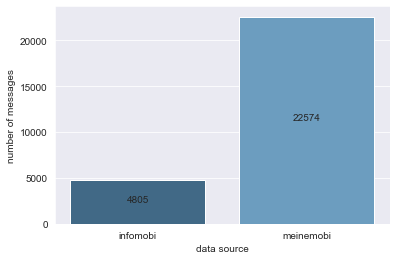
\includegraphics[scale=0.5]{plot-comparison-size}
    \caption{Size comparison of both data sources}
    \label{fig:plot-comparison-size}
\end{figure}

Figure \ref{fig:plot-comparison-size} shows, that the size of \emph{meinemobi} is more than four times larger than the size
of \emph{infomobi}. Before pre-processing there is a total number of 27 379 messages. This is a solid base if we
keep in mind, that a large part of the data may be removed at data cleansing. Afterwards, the remaining data needs to be
labelled manually to build a model by supervised learning techniques.

\subsection{Comparison}

There are large differences between these two data sets. The distribution of message types hugely varies between them.
As you can see in figure \ref{fig:plot-comparison-types}, about 80 percent of all messages are of type \emph{HTML}.
This is consistent among the two different data sources. More interesting is the fact, that \emph{infomobi} contains
more \emph{RTF} messages than \emph{Plain Text}, but very few of them are found in \emph{meinemobi}. This might be due to
the large number of spam inside \emph{infomobi} which is often formatted as \emph{RTF}. One possible reason for the spam could be,
that the generic email address of \emph{infomobi} is the victim of email harvesting\footnote{The discipline of obtaining email
addresses through various methods like patterns}.

In addition to junk mails, \emph{infomobi} contains a lot more messages in foreign languages than \emph{meinemobi}. These messages
must be removed, so the NLP model will only learn from German. A possible reason might be, that \emph{\textbf{info}@mobiliar.ch}
is more international than the language specific \emph{meinemobi} address. Consider chapter \ref{chap:cleansing} to see how
language detection is done.

\begin{figure}[!ht]
    \centering
    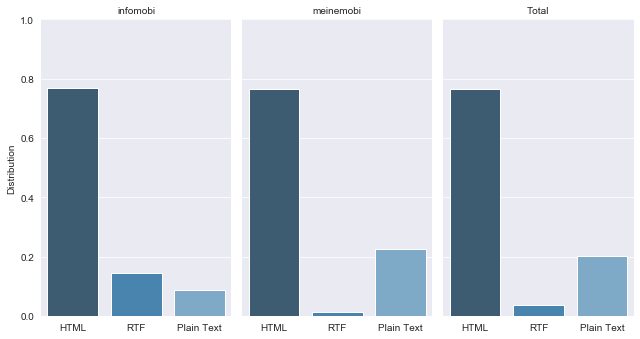
\includegraphics[scale=0.4]{plot-comparison-types}
    \caption{Distribution of the three message types}
    \label{fig:plot-comparison-types}
\end{figure}

Another important key figure is the typical length of a message. This key number can be measured in the total of words or
characters. Figure \ref{fig:plot-comparison-words} shows that the statistical mean of words is 196.

The division of the number of characters by the amount of words provides an idea about the typical word in this specific context.
Therefore the average word has a length of $8.45$ characters which is much higher than the average word in the \emph{\Gls{Duden}}
corpus with its length of $6.09$ characters \cite{duden}. Possible reasons might be the formal language used in the business
correspondence or insurance-related terms.

\begin{figure}[!ht]
    \begin{subfigure}{0.5\textwidth}
        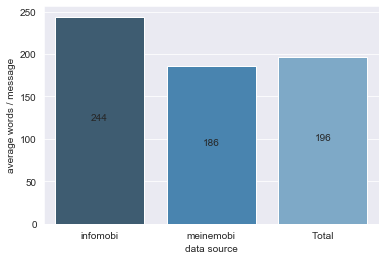
\includegraphics[scale=0.4]{plot-comparison-words} 
        \caption{Comparison of words}
        \label{fig:plot-comparison-words}
    \end{subfigure}
    \begin{subfigure}{0.5\textwidth}
        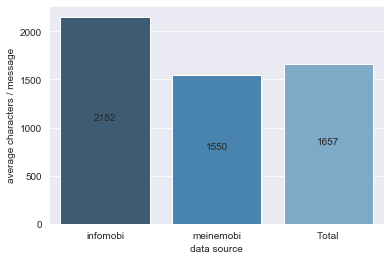
\includegraphics[scale=0.4]{plot-comparison-characters}
        \caption{Comparison of characters}
        \label{fig:plot-comparison-characters}
    \end{subfigure}
    \caption{Comparison of different indicators}
\end{figure}

\subsection{Typical Contents}
\label{chap:typical-contents}
Most messages can be divided into different groups. Such groups come very handy at the pre-processing stage when patterns should be
found to locate and remove junk from the remaining information. Therefore the mobi24 data can be splitted into several groups which
are best described with sample messages.

\subsubsection{Spam and Junk}

Junk mails are much harder to detect today than they used to be in the past. Nowadays they are well written and mostly grammatically
correct. Basically you could even use spam to train your model for certain use cases. But in that case spam should consistently be
removed from the data set because it lacks of the insurance context which the model should get familiar with. The presence of links,
the message length and the used language are often good indicators for detecting spam, especially when multiple indicators occur together.

\begin{quote}
    "Ein Ding der Unmöglichkeit! https://zixiseren1983.blogspot.in Auf Wiedersehen Elisabeth Speck"
\end{quote}

\begin{quote}
    "Hallo Ich bin Tony aus Indien. Wir sind ein Team von über 100 IT-Fachleuten mit Fachkenntnissen in folgenden Bereichen: Website-Design, Web-Entwicklung, PHP-Entwicklung, WordPress..."
\end{quote}

\begin{quote}
    "Mit der richtigen Haarpflege zur Traummähne :-) Die besten Pflegeprodukte für jeden Haartyp Endlich schöne Haare! Es ist Zeit, neue Haarprodukte zu entdecken..."
\end{quote}

\subsubsection{Auto-Generated Messages}

Some messages may not origin from real people but from machines instead. These group of messages is called \emph{automatically generated}
and represents the largest group of messages an usual human receives per day. In the data source there are newsletters, notifications
like payment success or delivery messages and failure reports present.

\begin{quote}
    "Fehler bei der Nachrichtenzustellung an folgende Empfänger oder Gruppen: generated1414@mobi.ch Die eingegebene E-Mail-Adresse konnte nicht gefunden werden..."
\end{quote}

\subsubsection{Customer Messages}

Moving forward, the messages which are actually written by humans and target Swiss Mobiliar's businesses are the only relevant
ones for the model. There's a wide range of message types like sponsoring requests, claim notifications, and technical questions.
All these messages share the same context.

Email messages are not as formal as letters and sometimes contain spelling errors. The texts are covered with typical Swiss expressions.
There are even Swiss Mobiliar specific words like the name of products, magazines or applications. It's important to train the future
model on this data to let it become aware of this typical kind of language.

\begin{quote}
    "Geschätzte Mobiliar ich habe mein Passwort verlegt. mit flotten Grüssen H. Muster"
\end{quote}

\begin{quote}
    "Guten Tag Im Anhang sende ich Ihnen die Offerte zum Schadenfall 8002.2533.9/XX zu. Wir bitten Sie die Offerte zu prüfen. Freundliche Grüsse Fritz Fischer"
\end{quote}

\begin{quote}
    "Liebe Mobiliar Ich möchte das Mobirama abbestellen. Freundliche Grüsse Hans M. Bundesgasse 35 3011 Bern"
\end{quote}

\section{Organisation}

This bachelor thesis is written during my last semester at the \acrlong{bfh} while I'm working full-time at the Swiss Mobiliar in
the Department of \emph{Cognitive Computing \& Disruptive Analytics}. The department is mainly responsible for the development of
cognitive applications to support existing business processes. The team is also driving the digital transformation and making
Swiss Mobiliar data addicted.

\subsection{Coordination}

Swiss Mobiliar is working with the \emph{Atlassian} tool stack. \emph{Jira} is used for keeping track of all tasks and dealing
with bug requests. The Kanban boards model the current project state by visualising the progress of each story or task.

I'm a member of the agile Scrum team \emph{Aare}\footnote{The beautiful river called Aare floats through the city of Berne}. Due
to the Scrum methodology, my colleagues are getting informed about my progress every morning at the daily scrum. At the end of each
sprint\footnote{At Swiss Mobiliar a sprint has a total duration of 3 weeks}, there is a Scrum activity called \emph{Sprint Review}
where I present my latest findings to the team.

\begin{figure}[!ht]
\centering
\frame{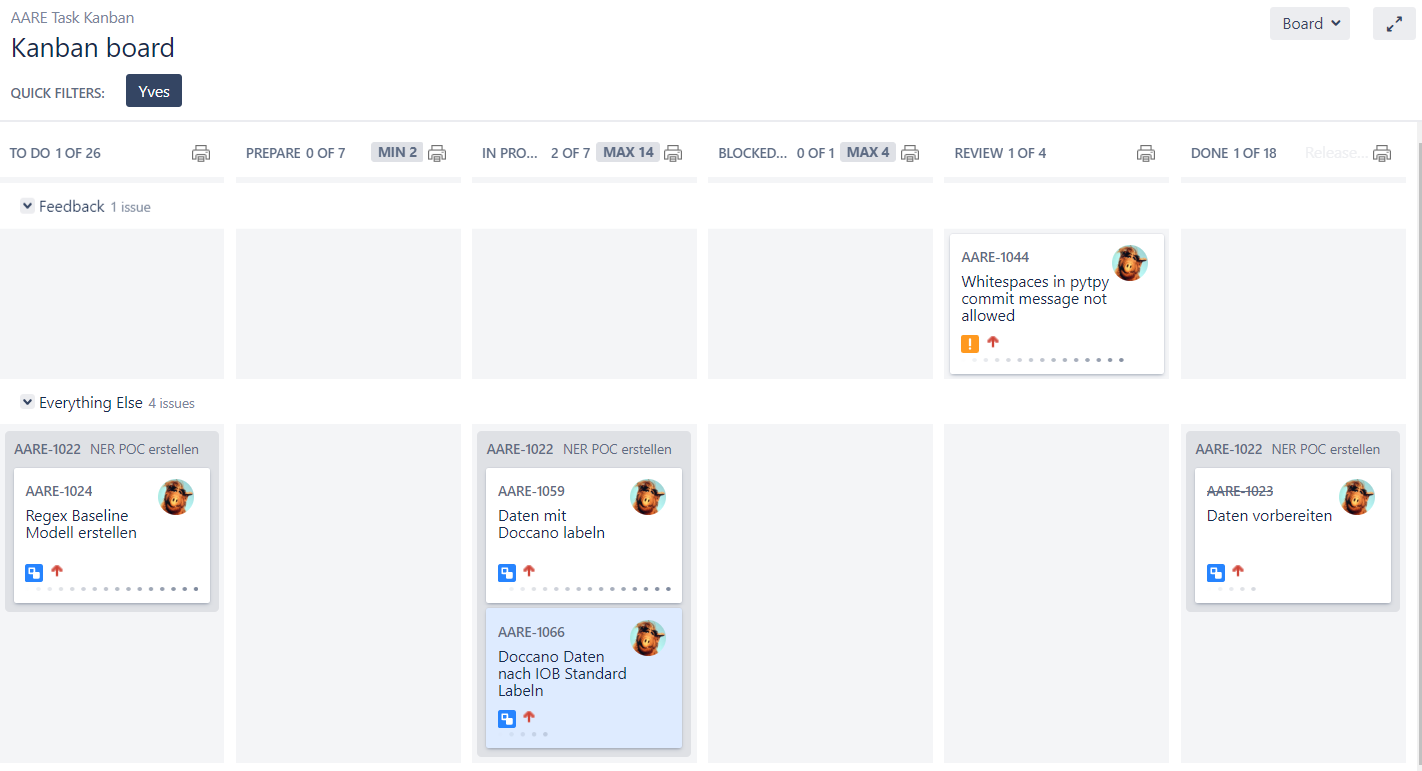
\includegraphics[width=\textwidth]{kanban}}
\caption{View of the Kanban board at an early project stage}
\label{fig:kanban}
\end{figure}

My supervising professor and I organise an informal meeting roughly every two weeks to discuss the project progress and to plan the
next steps. During this session I've got the time to ask questions concerning my current tasks. Due to the short time span between
these meetings, the project itself becomes very agile. I am able to change my primary focus to a different task within weeks.

\subsection{Development Environment}

All source code is generally written in Python. Small code snippets, mostly for exploring and mapping data into another structure,
are created with \emph{jupyter notebooks}. The models and larger pre-processing steps need to be robust and comprehensible, so
unit tests must be created. This code is under version control and is pushed frequently to the internal Git repository of
Swiss Mobiliar. Teamcity is used as a build server, which controls and deploys the code as a python library. To simulate later
applications, the model code is being run inside a docker container\footnote{Tool to run applications inside a container independent
of the underlying operating system}.

\chapter{Research}

This chapter gathers all research information together which is necessary to create and validate a functioning NLP model. This
isn't only about choosing the right algorithms for the task but also about finding ways to compare multiple approaches against
each other and validating their results.

\section{Performance Metrics}
\label{chap:formulas}
There exist several performance indicators each data scientist should be aware of. These specific metrics are used to validate
the outcome of models and make different solutions comparable. As in figure \ref{fig:metrics} displayed, there is a basic
concept which these metrics are build on top of.

\begin{figure}[!ht]
\centering
\frame{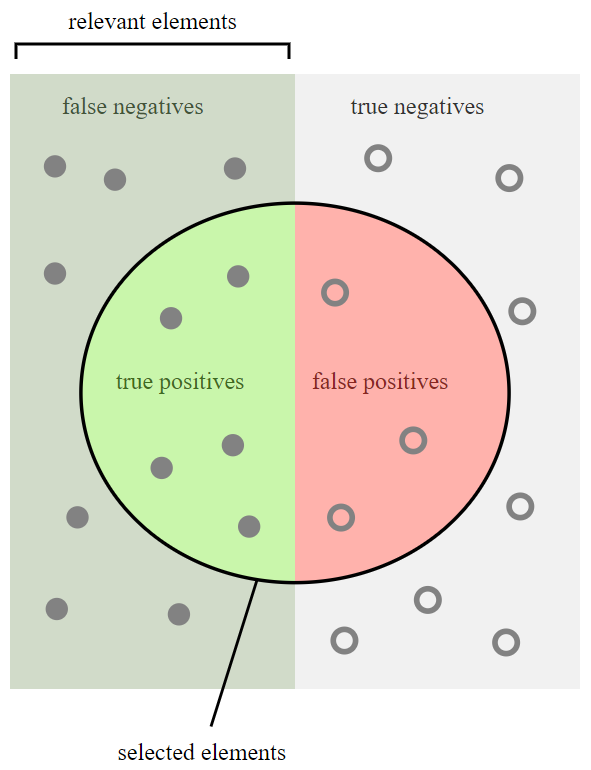
\includegraphics[scale=0.4]{metrics-overview}}
\caption{Overview about possible classification outcomes\cite{wiki01}}
\label{fig:metrics}
\end{figure}

For every binary classification task there exist exactly four possible outcomes. When the model classifies an element correctly it's
either a \emph{true positive} or a \emph{true negative} value. The keyword \emph{true} relates to the prediction the model did.
Vice versa it's either a \emph{false positive} or a \emph{false negative} value if the model's prediction is wrong.

The combination of \emph{true positive} and \emph{false negative} values is the amount of relevant data we want to have a closer
look at. For example this could be a set of \emph{named entities} or a group of patients which have a certain disease.

\subsection{Why Accuracy is not enough}
\label{chap:accuracy}
Probably the most well-known and certainly the easiest metric to understand is called \emph{accuracy}. It describes the
closeness of a set of predictions to its corresponding \emph{truth values}. Accuracy is the proportion of all correctly classified
elements in relation to the total quantity. It's value lies somewhere between zero and one.

\begin{equation}
    \label{math:accuracy}
    accuracy = \frac{\textit{true positives} + \textit{true negatives}}{\textit{total population}}
\end{equation}

There is one large downside with accuracy which makes it useless for many classification problems. If there's one category
representing the majority of elements, accuracy will always be at a very high level. This is called an \emph{imbalanced
classification problem} \cite{koehrsen}. Imagine a model for detecting very rare diseases which simply labels each tested patient
as \emph{negative}. If the chance of getting this disease is about \(\frac{1}{10000}\), the accuracy of such model would be at
stunning $99.99\%$. That's why every data scientist should consider using more advanced metrics as described in the next section.

\subsection{Precision and Recall}

\emph{Precision} measures the accuracy of the positive predictions. In other words, it's the proportion of correctly classified
elements in relation to all elements the model marked as \emph{positive}. A model which classifies only one single element as
\emph{positive} (the rest as \emph{negative}) and is right about that, will have a \emph{precision} of $1.0$. The results of a
model with a high \emph{precision} are very useful because most values have been correctly classified and therefore can be used
for further processing.

\begin{equation}
    \label{math:precision}
    precision = \frac{\textit{true positives}}{\textit{true positives} + \textit{false positives}}
\end{equation}

\emph{Recall}, or sometimes called \emph{sensitivity}, is the number of correct classifications compared to the number of elements
which should have been found in total. A \emph{recall} of $100\%$ can simply be achieved by classifying every element as \emph{positive}.
Therefore it should be combined with \emph{precision} to get an expressive statement about the model performance.

\begin{equation}
    \label{math:recall}
    recall = \frac{\textit{true positives}}{\textit{true positives} + \textit{false negatives}}
\end{equation}

There is a trade-off between the two metrics \emph{precision} and \emph{recall}. An optimization which increases the \emph{recall}
will likely decrease the \emph{precision} and vice versa. If neither \emph{recall} nor \emph{precision} is more important, there
exists the \emph{F1 score} (\ref{math:f1}) which is the harmonic mean of both. The mean itself isn't very meaningful because if the
model performs very good at one metric and poorly at the other, it will be still around $0.5$. The harmonic mean punishes low values
and doesn't compensate them with high values for the opposite metric. In many cases, \emph{F1 score} is a good metric to describe the
overall performance of a model \cite{Grus15}.

\begin{equation}
    \label{math:f1}
    \textit{f1 score} = 2 * \frac{precision * recall}{precision + recall}
\end{equation}

\section{Named-entity Recognition}

\acrfull{ner} is the first and probably most important discipline of \emph{information extraction}. Its goal is to detect
\emph{named entities} which is roughly everything that has a proper name. Sometimes this group is extended with terms like prices,
dates and times \cite{Jurafsky2000}. It's common to create own domain specific entities, e.g. an entity type \emph{insurance} which
might be useful for the Swiss Mobiliar. Table \ref{tbl:named-entities} shows typical named entity types which are supported by a
large variety of \acrshort{ner} libraries. \emph{Locations} and \emph{geo-political entities} are sometimes combined\footnote{The NLP
library spaCy combines these two for models trained by the Wikipedia corpus}.

\begin{table}[h!]
    \centering
    \begin{tabular}{|l|l|l|}
        \hline
        \textbf{Type} & \textbf{Tag} & \textbf{Description} \\ [0.5ex]
        \hline
        People & PER & People, Characters \\
        Organisation & ORG & Companies, NGOs, Sports \\
        Locations & LOC & Regions, Mountains, Seas \\
        Geo-Political Entity & GPE & Countries, Cities, Provinces \\ [1ex]
        \hline
    \end{tabular}
    \caption{List of generic named entity types}
    \label{tbl:named-entities}
\end{table}

Entities are used to recognise relations between people or for question answering like Google does\footnote{Simply google "who's
the mother of Zeus" where "Zeus" is a named entity}. Another possible use case is the automated grouping of news articles by
referenced people, organisations or locations \cite{gupta}.

\subsection{Difficulties}

In \acrlong{ner} it can be very difficult to decide what's a named entity and what's not. The term \emph{general agency Berne} can
refer to an organisation whereas the token \emph{Berne} could reference the capital of Switzerland. For the best possible results
it's important to define the boundaries of what's a named entity and what's not and to be strict while labelling.

Another difficulty is if you have to deal with word ambiguity. Imagine the entity \emph{Orange} which can either be a fruit, a colour,
a telecommunication provider or a city in France. Many fashion labels are named after designers like \emph{Calvin Klein} or \emph{Ralph
Lauren} but when people mention them, they mostly mean the brand rather than the actual person \cite{Vogel19}. The \acrshort{nlp} model
needs to consider the context in which the ambiguous term occurred to give a solid prediction.

\subsection{Labelling Standards}

Named entities need to be described in a standardised way so that \acrshort{ml} models can interpret them. There exist a few labelling
standards which are often used in \acrshort{ner}. If you have to chose a specific labelling standard, keep in mind that sophisticated
labelling techniques give you more information than e.g. binary labelling. You can always downgrade to a lower standard but getting
distinctive labels out of binary tags isn't possible. On the other hand, it's often easier to label data with low-level tags rather
than e.g. \acrshort{iob} tags.

\subsubsection{Binary}

Binary tagging is the simplest form of labelling. Every token which isn't a named entity is going to be labelled as $0$. The remaining
tokens which are all entities are tagged with $1$. If multiple label types need to be distinguishable, binary tagging isn't the preferred
method. As you can see in table \ref{tbl:binary-labelling}, the two entities \emph{people} and \emph{food} cannot be distinguished.

\begin{table}[h!]
    \centering
    \begin{tabular}{|c|c|c|c|c|c|c|c|}
        \hline
        Bond & drinks & his & vodka & martini & shaken, & not & stirred. \\
        \hline
        1 & 0 & 0 & 1 & 1 & 0 & 0 & 0 \\
        \hline
    \end{tabular}
    \caption{Example of a binary tagged sentence}
    \label{tbl:binary-labelling}
\end{table}

This issue can be solved by using multi-class labelling. This technique uses distinctive labels for every entity type as seen in
\ref{tbl:multiclass-labelling}.

\begin{table}[h!]
    \centering
    \begin{tabular}{|c|c|c|c|c|c|c|c|}
        \hline
        Bond & drinks & his & vodka & martini & shaken, & not & stirred. \\
        \hline
        1 & 0 & 0 & 2 & 2 & 0 & 0 & 0 \\
        \hline
    \end{tabular}
    \caption{Example of multi-class tagged sentence}
    \label{tbl:multiclass-labelling}
\end{table}

\subsubsection{IOB (Inside-outside-beginning)}

Unlike binary tags, \acrshort{iob} labels allow you to differentiate between multiple label types. \emph{Bond} and \emph{vodka martini}
are clearly not in the same entity group (\ref{tbl:iob-labelling}). Additional to the variable types, \acrshort{iob} tagging indicates
multi-token entities as such. In the \emph{IOB2} format, the first token of a sequence is always labelled with the prefix \emph{B-} for
beginning, the rest with an \emph{I-} for inside \cite{bio95}.

\begin{table}[h!]
    \centering
    \begin{tabular}{|c|c|c|c|c|c|c|c|}
        \hline
        Bond & drinks & his & vodka & martini & shaken, & not & stirred. \\
        \hline
        B-PER & O & O & B-FOOD & I-FOOD & O & O & O \\
        \hline
    \end{tabular}
    \caption{Example of an IOB tagged sentence}
    \label{tbl:iob-labelling}
\end{table}

As shown in table \ref{tbl:iob-labelling2}, the first two tokens are from the same type but still distinguishable. With binary tags you
would most likely interpret both tokens as one large named entity consisting of two separate words.

\begin{table}[ht!]
    \centering
    \begin{tabular}{|c|c|c|c|c|c|}
        \hline
        Huey, & Dewey, & and & Louie & are & triplets. \\
        \hline
        B-PER & B-PER & O & B-PER & O & O \\
        \hline
    \end{tabular}
    \caption{Example of distinctive beginning tags}
    \label{tbl:iob-labelling2}
\end{table}

\subsubsection{BIOES}

The \acrshort{iob} format was later extended by an indicator for single and ending tokens. It's called \emph{BIOES} and can be useful if
tokens are processed separately from each other so that the model cannot be able to recognise multi-token values by itself.
The \emph{s} stands for single tokens whereas the \emph{e} indicates ending tokens \cite{hofer18}.

\begin{table}[h!]
    \centering
    \begin{tabular}{|c|c|c|c|c|c|c|c|}
        \hline
        Bond & drinks & his & vodka & martini & shaken, & not & stirred. \\
        \hline
        S-PER & O & O & B-FOOD & E-FOOD & O & O & O \\
        \hline
    \end{tabular}
    \caption{Example of an BIOES tagged sentence}
    \label{tbl:bioes-labelling}
\end{table}

\chapter{Approaches}

\section{Pre-processing}

\subsection{Data Cleansing}

Insert table width key values before and after cleansing:

infomobi: before = 12420, after = 3259
etc..

\section{Baseline Models}

\subsection{SpaCy Library}

\subsubsection{Performance}

Values for NER only with PER:
    Accuracy 0.9604750950612733
    Precision 0.45423386721729264
    Recall 0.5127429916103949
    
Values for NER with LOC:
	Accuracy 0.9702884543615491
	Precision 0.05402757788198153
	Recall 0.03206319974275776




% glossary
\printglossaries

% bibliography
\bibliographystyle{plain}
\bibliography{references}

% appendix
\appendix
\chapter{Resources}

This chapter contains code snippets, performance measurements, and additional information which would unnecessarily bloat the report. Only the important parts are covered in this section. The complete source code was handed to the supervising professor before the submission deadline.

\section{Performance Metrics}

The \acrlong{kpi}s are measured with a total of 967 manually-labelled messages. These numbers will be affected by adding more trainig samples. Consider section \ref{chap:formulas} for more information about the different \acrshort{kpi}s.

\subsection{SpaCy}

\begin{table}[ht!]
    \centering
    \begin{tabular}{|p{6em}|p{3em}|}
        \hline
        Accuracy & 0.946 \\
        \hline
        Precision & 0.444 \\
        \hline
        Recall & 0.533 \\
        \hline
        \textbf{F1 Score} & \textbf{0.485} \\
        \hline
    \end{tabular}
    \caption{Spacy KPIs}
    \label{tbl:perf-spacy}
\end{table}

\begin{table}[ht!]
    \begin{minipage}{.5\linewidth}
        \centering
        \begin{tabular}{|p{6em}|p{3em}|}
            \hline
            Accuracy & 0.955 \\
            \hline
            Precision & 0.405 \\
            \hline
            Recall & 0.685 \\
            \hline
            \textbf{F1 Score} & \textbf{0.509} \\
            \hline
        \end{tabular}
        \caption{Spacy (only PER)}
        \label{tbl:perf-spacy-per}
    \end{minipage}%
    \begin{minipage}{.5\linewidth}
        \centering
        \begin{tabular}{|p{6em}|p{3em}|}
            \hline
            Accuracy & 0.933 \\
            \hline
            Precision & 0.039 \\
            \hline
            Recall & 0.158 \\
            \hline
            \textbf{F1 Score} & \textbf{0.063} \\
            \hline
        \end{tabular}
        \caption{Spacy (only LOC)}
        \label{tbl:perf-spacy-loc}
    \end{minipage}
\end{table}

\subsection{Basic Lookup Model}

Consider chapter \ref{chap:regex-model} for more information about the different enhancements.

\begin{table}[ht]
    \centering
    \begin{tabular}{|L{16em}|C{3em}|C{3em}|C{3em}|C{3em}|}
        \hline
        \textbf{Enhancement} & \textbf{Acc} & \textbf{Prec} & \textbf{Rec} & \textbf{F1} \\ [1ex]
        \hline
        1 - Add dictionary lookup & 0.774 & 0.146 & 0.733 & 0.243 \\ [0.2ex]
        \hline
        2 - Remove last names dictionary & 0.953 & 0.582 & 0.401 & 0.475 \\ [0.2ex]
        \hline
        3 - Clean up last names & 0.948 & 0.432 & 0.723 & 0.541 \\ [0.2ex]
        \hline
        4 - Add uppercase constraint & 0.953 & 0.487 & 0.722 & 0.582 \\ [0.2ex]
        \hline
        5 - Escape \gls{diacritic}s & 0.953 & 0.486 & 0.736 & 0.585 \\ [0.2ex]
        \hline
        6 - Add variants (e.g. umlauts) & 0.952 & 0.503 & 0.758 & 0.605 \\ [0.2ex]
        \hline
        7 - Add previous and next tokens & 0.954 & 0.504 & 0.761 & 0.606 \\ [0.2ex]
        \hline
        8 - Clean up first- and last names & 0.982 & 0.773 & 0.752 & 0.762 \\ [0.2ex]
        \hline
        9 - Replace addresses with regex & 0.98 & 0.848 & 0.732 & \textbf{0.786} \\ [0.2ex]
        \hline
    \end{tabular}
    \caption{Basic Lookup Model KPIs}
    \label{tbl:perf-regex}
\end{table}

\begin{table}[ht!]
    \begin{minipage}{.5\linewidth}
        \centering
        \begin{tabular}{|p{6em}|p{3em}|}
            \hline
            Accuracy & 0.984 \\
            \hline
            Precision & 0.737 \\
            \hline
            Recall & 0.885 \\
            \hline
            \textbf{F1 Score} & \textbf{0.804} \\
            \hline
        \end{tabular}
        \caption{Lookup Model (PER)}
        \label{tbl:perf-regex-per}
    \end{minipage}%
    \begin{minipage}{.5\linewidth}
        \centering
        \begin{tabular}{|p{6em}|p{3em}|}
            \hline
            Accuracy & 0.951 \\
            \hline
            Precision & 0.111 \\
            \hline
            Recall & 0.334 \\
            \hline
            \textbf{F1 Score} & \textbf{0.166} \\
            \hline
        \end{tabular}
        \caption{Lookup Model (LOC)}
        \label{tbl:perf-regex-loc}
    \end{minipage}
\end{table}

\subsection{Deep Learning}

Here are the metrics for the very deep net and stuff..

\section{Source Code}

\subsection{Keras Tokenizer}

The Keras tokenizer allows you to define the \emph{OOV} token during initialisation. With the \verb|filter| option you can define which characters the tokenizer should filter from the tokens. The default filter would handle "\emph{Hello}" and "\emph{Hello,}" as the same token. For not losing punctuation the \verb|filter| parameter needs to be set to an empty string.

\begin{lstlisting}[language=Python, label={code:keras-tokenizer}, caption=Fitting the Keras tokenizer]
from tensorflow.keras.preprocessing.text import Tokenizer

tokenizer = Tokenizer(oov_token='<OOV>', filters='')

# create a vocabulary based on the training set
tokenizer.fit_on_texts(train_sentences)

# create sequences of IDs
sequences = tokenizer.texts_to_sequences(test_sentences)
\end{lstlisting}

\subsection{Sliding Window}

\begin{lstlisting}[language=Python, label={code:sliding-window}, caption=Sliding window implementation]
def sliding_window(sequences, window_size=5, placeholder='', flatten=True):
    """
    Creates windows of the exact same size, first and last windows
    will be padded with a placeholder. The relevant token of each
    window is placed in the middle. Flattens the list by default.
    """
    half = int(window_size / 2)
    results = []

    for sequence in sequences:

        tokens = sequence[0]
        labels = sequence[1]

        length = len(tokens)
        windows = []

        # create windows
        for idx in range(length):
            start = idx - half
            stop = idx + 1 + half
            windows.append([tokens[max(0, start):stop], labels[idx]])

        # add padding for first windows
        for idx, val in enumerate(range(half, 0, -1)):
            tmp = windows[idx][0]
            for i in range(val):
                tmp = [placeholder] + tmp

            windows[idx][0] = tmp

        # add padding for last windows
        for val, idx in enumerate(range(length-half, length)):
            tmp = windows[idx][0]
            for i in range(val+1):
                tmp = tmp + [placeholder]

            windows[idx][0] = tmp

        results.append(windows)

    if flatten:
        results = [item for sublist in results for item in sublist]

    return results
\end{lstlisting}

\section{Miscellaneous}

\subsection{Excluded Ambiguous Names}
\label{lst:excluded-names}

The following list shows all values which aren't common names or which may be names but are ambiguous. These values are removed from the naming dictionaries which are used by the regex baseline model.

\begin{multicols}{4}
    \begin{itemize}
        \item mobiliar
        \item mobi
        \item immobilien
        \item safari
        \item franken
        \item guten
        \item leider
        \item min
        \item link
        \item weiss
        \item herr
        \item app
        \item kunde
        \item dame
        \item damen
        \item frau
        \item gerne
        \item sport
        \item firma
        \item herren
        \item liebe
        \item schaden
        \item grund
        \item person
        \item kinder
        \item mio
        \item juni
        \item bern
        \item mail
        \item post
        \item mar
        \item sun
        \item fall
        \item ort
        \item hand
        \item mon
        \item wed
        \item may
        \item gruss
        \item abend
        \item mai
        \item juni
        \item juli
        \item phone
        \item spray
        \item buchung
        \item freitag
        \item montag
        \item monday
        \item fehler
        \item glueck
        \item uri
        \item seite
        \item auto
        \item pin
        \item biel
        \item you
        \item helvetia
        \item weg
        \item art
        \item termine
        \item chance
        \item merci
        \item stecker
        \item preis
        \item partner
        \item restaurant
        \item handy
        \item zurich
        \item schlechten
        \item privat
        \item frische
        \item kan
        \item name
    \end{itemize}
\end{multicols}



\end{document}
